\subsection{Технология сборки платы управления}
\subsubsection{Анализ особенностей конструкции платы}
Плата управленияс параметрами (см. таблицу \ref{comon_board_param})
с размещёнными на ней электрорадиоэлементами (далее ЭРЭ) преобладающее
большинство из которых планарного монтажа.

\begin{table}[ht!]
    \centering
    \begin{tabular}{|l|c|}
        \hline
        Наименование & значение \\
        \hline
        Габаритные размеры, мм. & 72x120x15 \\
        Шаг координатной сетки, мм. & 0.4 \\
        Минимальное расстояние между продниками, мм. & 0.2 \\
        Класс точности платы & 3 \\
        Общее количество элементов, шт. & 155 \\
        Количество наименований элементов, шт. & 61 \\
        Количество выводных элементов, шт. & 12 \\
        Количество \textit{SMD} элементов, шт. & 143 \\
        Количество разъемов, шт. & 6 \\
        \hline
    \end{tabular}
    \caption{Основные параметры платы}
    \label{comon_board_param}
\end{table}

Особенностями конструкции, существенными с точки зрения технологического
процесса сборки платы блока управления, являются:
\begin{itemize}
    \item Односторонняя печатная плата
    \item Высокая повторяемость типоразмеров ЭРЭ
    \item Коммутация с другими элементами конструкции осуществляется c помощью
        кабелей, подключаемых через штыревые разъемы
    \item ЭРЭ располагаются с одной стороны печатной платы
    \item В числе ЭРЭ есть не только \textit{SMD} компоненты, но и выводные
        (6 выводных конденсаторов и 6 разъёмов) пайки оплавлением будет
        недостаточно.
\end{itemize}

\subsubsection{Разработка маршрутной технологии монтажа}
Разработка технологии монтажа ПП основана на требованиях по
безопасности изготовления платы и требованиях по термоустойчивости
элементов и самой печатной платы.
Основными критериями для получения работоспособной печатной
платы являются время и температура пайки, лужения и флюсования выводов
различных элементов.

\paragraph{Оборудование для сборки}
Преобладющее большинство устанавливаемых компонентов --- планарного монтажа,
поэтому основной способ сбоки платы - это пайка оплавлением. Для этого была
выбрана паяльная паста на безсвинцовом припое с флюсом не требующим отмывки
\textit{Indium NC-SMQ 92J}.
Так же имется небольшое количество выводных компонентов, которые паяются
волной припоя. Устанавливаются перед этим вручную на плату.
Перед нанесение пасты, плату необходимо промыть от технологических загрязнений.

\begin{itemize}
    \item Установка для отмывки печатных плат \textit{Радуга-60.2}. Для промывки
            платы от технологических загрязнений.
    \item Автоматический трафаретный принтер \textit{P500}. Для нанесения
            паяльной пасты на посадочные площадки платы для \textit{SMD}
            компонентов.
    \item Установщик компонентов \textit{SMT2000 IVAS tech}. Для установки
            \textit{SMD} компонентов на паяльную пасту.
    \item Конвекционная конвейерная печь \textit{BM745}. Для оплавления паяльной
            пасты под \textit{SMD} компонентами.
    \item Монтажный стол. Для ручной установки выводных компонентов перед пайкой
            волной припоя, для покрытия платы финишных покрытий.
    \item Установка пайки двойной волной припоя \textit{WS-400F}. Для пайки
            выводных компонентов.
\end{itemize}

В результате процесс монтажа платы управления состоит из:
\begin{enumerate}
    \item Очистка печатной платы
    \item Нанесение паяльной пасты
    \item становка SMD компонентов на пасту
    \item Пайка оплавлением
    \item Установка выводных компонентов
    \item Пайка волной
    \item Очистка печатной платы
    \item Нанесение финишного покрытия
\end{enumerate}

Подробнее маршрутную карту смотри в приложении.

\subsubsection{Оценка технологичности конструкции платы}
На плате расположено много разнородных элементов, некоторые из которых
устанавливаются в единственном экземпляре, что значительно снижает
технологичность монтажа.
Однако при разработке учитывались некоторые факторы технологичности, и поэтому
применяется всего двухслойная печатная плата с установкой элементов с планарными
выводами (за исключением электролитических конденсаторов и разъемов).
Плата разведена с шагом координатной сетки 0.5 мм.
Установленные на плату компоненты и количесвто выводов им соотвествующее,
сгруппированные по функциональному назначению перечислены в таблице
(\ref{components_and_mount_points}).

\begin{table}
    \centering
    \begin{tabu}{|X[-1,l,m]|X[-1,c,m]|X[c,m]|}
        \hline
        Название & Количество, шт & Общее количество выводов, шт \\ \hline
        Микросхемы & 9 & 180 \\ \hline
        Чип резисторы & 64 & 128 \\ \hline
        Чип конденсаторы & 51 & 102 \\ \hline
        Электролитические конденсаторы & 6 & 12 \\ \hline
        Чип светодиоды & 7 & 14 \\ \hline
        Разъемы & 6 & 33 \\ \hline
        Чип индуктивность & 1 & 2 \\ \hline
        Чип стабилитрон & 1 & 2 \\ \hline
    \end{tabu}
    \caption{Установленные на плату компоненты по количеству выводов}
    \label{components_and_mount_points}
\end{table}

Исходные данные для определения комплексного показателя технологичности
приведены в таблице (\ref{technological_estaime_parametres}).

\begin{table}
    \centering
    \begin{tabu}{|X[l,m]|X[-1,c,m]|X[-1,c,m]|} \hline
        Исходные данные & Обозначения & Значение \newline показателя \\ \hline
        Количество монтажных соединений, которые могут осуществляться
        механизированным или автоматизированным способом,
        т.е. имеются механизмы, оборудование или оснащение для
        выполнения монтажных соединений.
        % все кроме тех, что устанавливаем вручную, электролит. конд. и разъемы
        & $H_{\text{ам}}$ & 473  \\ \hline
        Общее количество монтажных соединений
        % полное количество ножек
        & $H_{\text{м}}$ & 473  \\ \hline
        Общее количество микросхем в блоке & $H_{\text{мс}}$ & 9  \\ \hline
        Общее количество ЭРЭ & $H_{\text{ЭРЭ}}$ & 136  \\ \hline
        Количество ЭРЭ, подготовка которых к монтажу осуществляется (может
        осуществляться) механизированным или автоматическим способом,
        т.е. имеются механизмы, оборудование или оснащение для выполнения
        монтажных соединений.
        % все кроме тех, что устанавливаем вручную, электр. конд. и разъемы
        & $H_{\text{мп ЭРЭ}}$ & 123  \\ \hline
        Количество операций контроля и настройки, которые можно осуществить
        автоматизированным или механизированным способом.
        & $H_{\text{мкн}}$ & 0  \\ \hline
        Общее количество операций контроля и настройки
        & $H_{\text{кн}}$ & 2  \\ \hline
        Общее количество типоразмеров ЭРЭ в изделии
        & $H_{\text{т ЭРЭ}}$ & 22  \\ \hline
        Количество типоразмеров оригинальных ЭРЭ в изделии
        & $H_{\text{тор ЭРЭ}}$ & 0  \\ \hline
    \end{tabu}
    \caption{Показатели технологичности}
    \label{technological_estaime_parametres}
\end{table}

Коэффициент использования микросхем и транзисторных матриц в блоке.
Весовой коэффициент $\phi = 1$.
$$
K_{\text{испмс}}
    = \frac{H_\text{мс}}
           {H_\text{ам}}
    = \frac{9}{473}
    = 0.019027
$$

Коэффициент автоматизации и механизации монтажа.
Весовой коэффициент $\phi = 1$.
$$
K_{\text{гсм}}
    = \frac{H_\text{ам}}
           {H_\text{м}}
    = \frac{473}{473}
    = 1
$$

Коэффициент механизации подготовки ЭРЭ.
Весовой коэффициент $\phi = 0.75$.
$$
K_{\text{мс}}
    = \frac{H_\text{мп ЭРЭ}}
           {H_\text{ЭРЭ}}
    = \frac{123}{136}
    = 0.904412
$$

Коэффициент механизации контроля и настройки.
Весовой коэффициент $\phi = 0.5$.
$$
K_\text{кмн}
    = \frac{H_\text{мкн}}
           {H_\text{кн}}
    = \frac{0}{2}
    = 0
$$

Коэффициент повторяемости ЭРЭ.
Весовой коэффициент $\phi = 0.31$.
$$
K_\text{повЭРЭ}
    = 1 - \frac{H_\text{т ЭРЭ}}
               {H_\text{ЭРЭ}}
    = 1 - \frac{22}{136}
    = 0.838235
$$

Коэффициент применяемости ЭРЭ.
Весовой коэффициент $\phi = 0.187$.
$$
H_{\text{МКН}}
    = 1 - \frac{H_\text{тор ЭРЭ}}
               {H_\text{т ЭРЭ}}
    = 1 - \frac{0}{22}
    = 1
$$

Определение комплексного показателя технологичности.
$$
\sum_{i=1}^6 K_i \cdot \phi_i =     1 \cdot 0.019027
                                +   1 \cdot 1
                                +   0.75 \cdot 0.904412
                                +   0.5 \cdot 0
                                +   0.31 \cdot 0.838235
                                +   0.187 \cdot 1
$$

$$
\sum_{i=1}^6 \phi_i = 1 + 1 + 0.75 + 0.5 + 0.31 + 0.187
$$

$$
K   = \frac{\sum_{i=1}^6 K_i \cdot \phi_i }
        {\sum_{i=1}^6 \phi_i }
    = 0.572241
$$

Норматив комплексных показателей устанавливает ОСТ4 ГО.091.219 \cite{OST4_GO_010_011}.
В соответствии с данным ОСТ комплексный показатель технологичности электронных
блоков автоматизированных систем управления и электронно--~вычислительной техники,
выпускаемой серийно, находится в пределах:

\begin{itemize}
    \item установочная серия --- К = 0.25...0.5
    \item установившееся серийное производство --- К = 0.3...0.6
\end{itemize}

Таким образом, изделия отвечают требованиям технологичности в условиях
серийного производства.

\subsubsection{Стенд проверки платы управления}
Схема стенда проверки работоспособности платы управления мехатронным модулем
изображена на рис (\ref{pcb_technology_check_stand}).

\begin{figure}
    \centering
    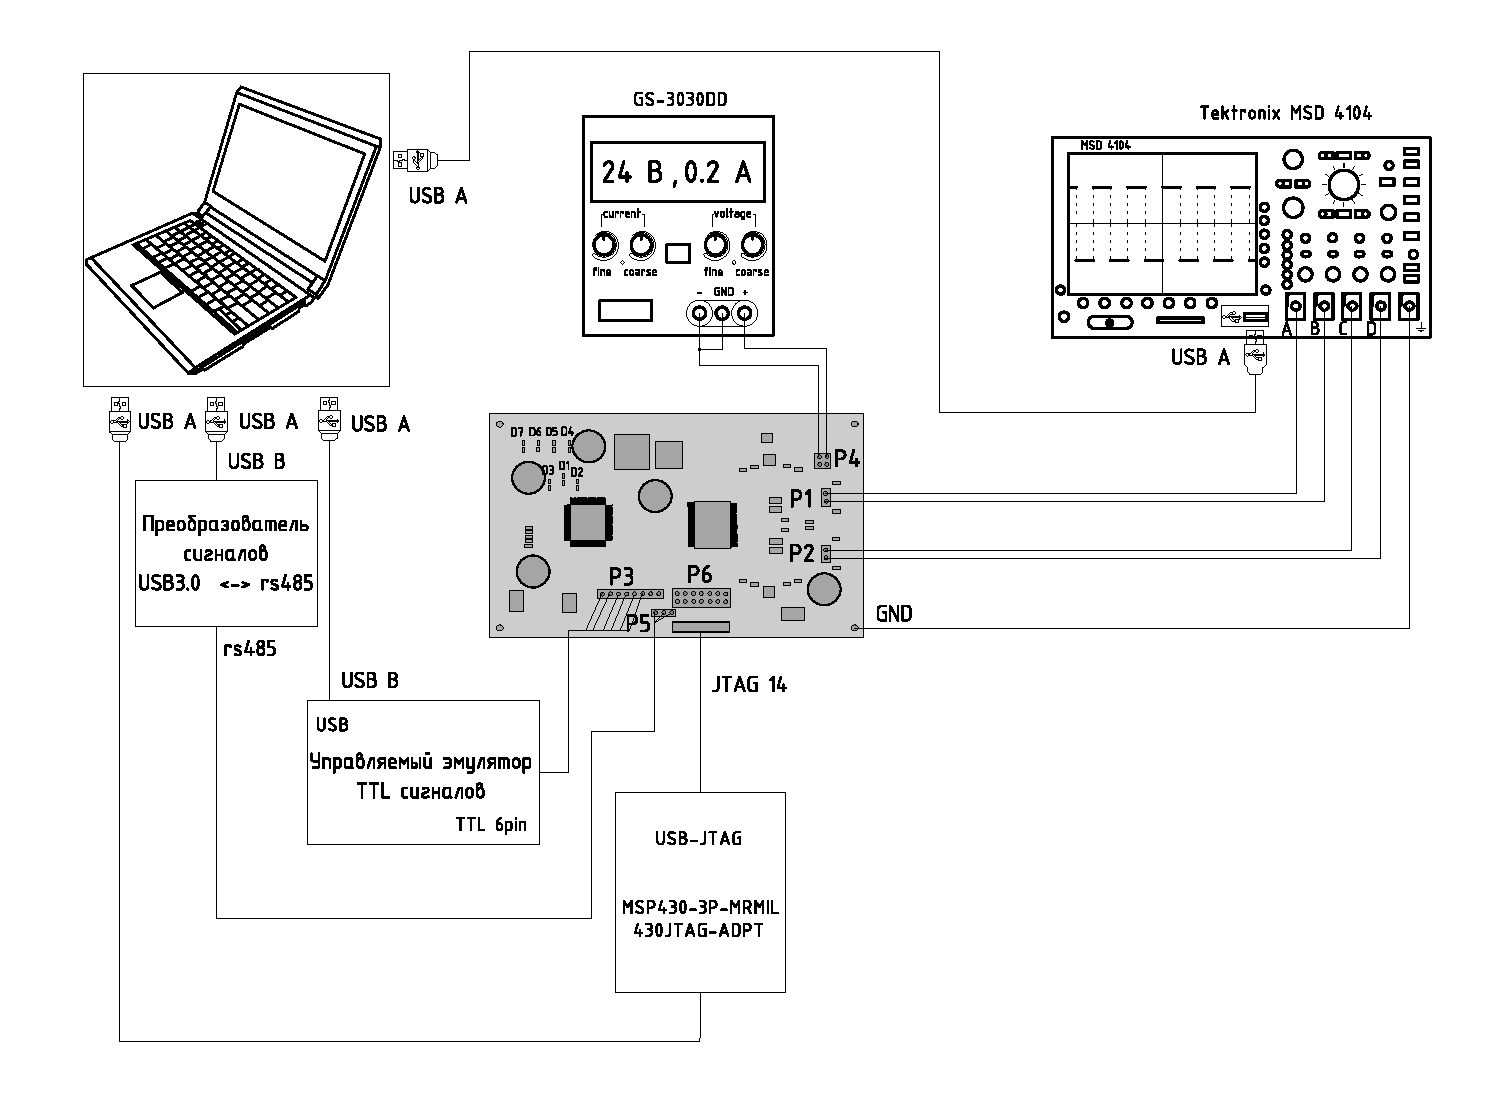
\includegraphics[   width=1.3\textwidth, angle=90, keepaspectratio, clip=true,
                        trim=1cm 1cm 1cm 0.6cm
                    ]
                    {src/pictures/pcb_technology_check_stand_rpz_ver}
    \caption{Стенд проверки работоспособности платы управления}
    \label{pcb_technology_check_stand}
\end{figure}

Состав схемы:
\begin{enumerate}
    \item Лабораторный источник питания
    \item ЭВМ
    \item Преобразователь сигналов USB --- rs485
    \item Программатор MSP430--3P--MRMIL
    \item Осцилограф Tektronix MSD 4104
    \item Управляемый эмулятор TTL сигналов
    \item Плата управления мехатронного модуля
    \item Кабель USB A --- USB A
    \item Кабель USB A --- USB B: 3 шт.
    \item Кабель питания платы управления мехатронным модулем
        MF-2x2 MRA - MATE-N-LOK
    \item Кабель сигнальный MF-2x1 --- 2--RG-59 (HYR-0101B): 2 шт.
    \item Кабель CWF-8 (DS1069-8 M) --- CWF-8 (DS1069-8 M)
    \item Кабель B3B-EH-A B3B-EH-B
\end{enumerate}


\textbf{Работоспособность} --- это состояние объекта или субъекта, при котором он
способен выполнять заданную функцию с параметрами, установленными требованиями
технической документации.


\textbf{Отказ} --- это нарушение работоспособности.

Работоспособной считаем плату, в которой функционируют все основные системы,
а именно:
\begin{itemize}
    \item Шина питания \textit{+12 В}
    \item Шина питания \textit{+5 В}
    \item Шина питания \textit{+3.3 В}
    \item Микроконтролер
    \item Связь по интерфейсу rs485
    \item Драйвер
    \item Энкодер
\end{itemize}
Работоспорособность преобразователей пинтания прверяем по состоянию светодиодов
D7, D6, D5, D4. Работоспособность цепей микроконтролера и его самого проверяем
по индикации его светодиодов D1, D2, а также по способности прошиваться по
интерфейсу JTAG.

Далее проверяем работоспособность интерфейса rs485 по
возможности обмена информацией по интрфейсу rs485. На номинальной частоте обмена
115200. Производится эхо~--~тест сообщениями с случано подобранным набором
символов длинной 250 байт. При совпадении исходящей и входящей
последовательностей считаем что тест пройден.

Проверка драйвера сводится к проверке корректности отработки различных уровней
ШИМ, они задаются посредсвом сообщений по интерфейсу rs485. Снятие сигнала и
оцифровывание осуществляется посредством электронного осцилографа, далее сигнал
через встроенный интерфейс через USB снимается ЭВМ, где и происходит сравнение
с эталоном. На основе сравнение выносится решение о работоспособности драйвера.

Проверка энкодера используя генератора TTL логики эмулирует корректный сигнал
энкодера на 550 единиц, запрашивает реально посчитанное платой значение, они
должны совпадать.

В итоге проверка на работоспособность включает в себя 3 визуальных теста, 4
автоматизированных. И представляет собой следующую последовательность действий:

\begin{enumerate}
    \item Собрать стенд по схеме
    \item Включить осцилограф и ЭВМ
    \item Подать напряжение \textit{24 В} на плату управления мехатронным
            модулем от лабораторного источника питания
    \item Убедиться, что потребляемый платой ток не превышает 0.2 А
    \item Проконтролировать визуально свечение светодиодов D4 (белый),
            D5 (желтый), D6 (зеленый), D7 (оранжевый).
    \item Загрузить тестовое программное обеспечение в память микроконтроллера,
            запустив скрипт ``firmware\_update'', убедиться что код ошибки ``0''
    \item Отсоединить шлейф программатора, перезагрузить плату, отключением и
            включением питания
    \item Проконтролировать свечение светодиодов D1 (зеленый) и D2 (голубой)
    \item Запустить скрипт тестирования интерфейса связи ``net\_test'',
            убедиться что, возвращаемый код ошибки ``0''
    \item Запустить скрипт проверки усилителя мощности ``pwm\_test'', убедиться,
            что возвращаемый код ошибки ``0''.
    \item Запустить программу проверки энкодера ``encoder\_test'', убедиться,
            что возвращаемый код ошибки ``0''.
    \item Убедиться что, светодиоды D1, D2, D4, D5, D6, D7 продолжают непрерывно
            светиться
    \item Выключить иточник питания, осцилограф, ЭВМ
\end{enumerate}
